\chapter{Ciclos de refrigeración}

\vspace{\fill}

\hrule

\vspace{.3cm}

{\large \lipsum[1]} 

\pagestyle{fancy}

\newpage

\section{Parámetros principales de ciclos}
\Biblio{\cite[pág. 21 a 22, 126 a 127]{Cengel2012termodinamica} \cite[pág. 48, 103, 254]{Rajput2011termodinamica}}

\subsection{Presión}

\begin{defs}
    La \textbf{presión} $(p)$ se define como una fuerza normal que ejerce un fluido por unidad de área.
\end{defs}

La presión real en una determinada posición se llama presión absoluta, y se mide respecto al vacío absoluto. Sin embargo, la mayor parte de dispositivos para medir la presión se calibran a cero en la atmósfera, por lo que indican la diferencia de presión absoluta y la presión atmosférica local, denominada presión manométrica ($P_{man}$). Las presiones por debajo de la presión atmosférica se denominan presiones de vacío ($P_{vac}$) y se miden mediante medidores de vacío que indican la diferencia entre las presiones atmosféricas y absoluta. Las presiones absoluta, manométrica y de vacío son todas positivas y se expresan como:

\begin{equation}\label{EA1-Relación de presiones}
    p_{man} = p_{abs} - p_{atm} \hspace{2cm} p_{vac} = p_{atm} - p_{abs}
\end{equation}


Puesto que la presión se define como la fuerza por unidad de área, tiene como unidad el Newton por metro cuadrado, también conocida como pascal.

\begin{equation}\label{EA1-Presión unidades}
    1 Pa = 1N/m^2
\end{equation}

Sin embargo, como esta unidad es muy pequeña, suele expresarse como kilopascal ($KPa$) o megapascal ($MPa$).

Además, fuera del sistema internacional de unidades, se presentan las unidades de presión bar, atmósfera y kilogramos fuerza por centímetro cuadrado. Estos valores presentan la siguiente relación:

\begin{equation}\label{EA1-Relación entre unidades}
    1atm \equiv 101.325KPa \equiv 1.01325bar \equiv 1.033kg/cm^2 \equiv 14.7psi
\end{equation}


\subsection{Energía interna}

\begin{defs}
    La \textbf{energía interna} $(u)$ es aquella energía térmica almacenada de un fluido.
\end{defs}

La energía interna es un termino que difiere de la energía mecánica, eléctrica, o química, y que está relacionada directamente con la energía térmica de un fluido. Su valor absoluto no se determina con facilidad. Sin embargo, en la ingeniería, la variación de la energía interna resulta un dato de mayor relevancia y fácil de determinar.

Como se verá más adelante, las variaciones de energía interna pueden relacionarse con las variaciones de temperatura según su calor específico en diferentes condiciones. Las dos condiciones principales son a volumen constante y a presión constante, llegando a que:

\begin{equation}
    \Delta u = c_p \Delta T \hspace{2cm} \Delta u = c_v \Delta T 
\end{equation}

siendo $c_p$ y $c_v$ los calores específicos a presión y volumen constante respectivamente; valores que indican la cantidad de energía necesaria para aumentar un grado la temperatura del fluido.

La energía interna en el sistema internacional es expresada en unidades de Joules.

\begin{equation}\label{EA1-Energía interna unidades}
    J = Kg \, m^2/s^2
\end{equation}

Otra unidad presente en la medición de energía interna es la caloría, donde la relación entre Joules y calorías es la siguiente:

\begin{equation}\label{EA1-Energía interna Relación entre unidades}
    4.184 J \equiv 1cal
\end{equation}


\subsection{Entropía}

\begin{defs}
    La \textbf{entropía} $(s)$ es un parámetro que define la cantidad de calor capaz de convertirse en trabajo. Mientras menor es la temperatura de un fluido, mayor será su entropía para la misma variación de calor.

    \begin{equation}\label{EA1-Entropía}
        ds = \dfrac{dQ}{T}
    \end{equation}
\end{defs}

La entropía, al ser un parámetro que relaciona el calor y la temperatura a partir de la integral, permite determinar el flujo de calor entre dos estados como:

\begin{equation}
    Q_{1\rightarrow2} = \int_{1}^{2} dQ = \int_{1}^{2} T(s) \, ds 
\end{equation}

Donde, si se emplea una gráfica $T-s$, gráfica muy común en análisis de refrigeración, es posible determinar el calor utilizado en los procesos y determinar trabajos realizados por dispositivos a partir de diferencias de áreas\footnote{Para ello es fundamental conocer los conceptos matemáticos de integral y la 2° Ley de la termodinámica.}.

La entropía, en el sistema internacional, se expresa en Joules sobre kelvin.

\begin{equation}\label{EA1-entropía Relación entre unidades}
    J/K = Kg \, m^2 /(s^2 K)
\end{equation}

\subsection{Entalpía}


\begin{defs}
    La \textbf{entalpía} $(h)$ es la relación, determinada por conveniencia y simplificación, entre la presión, la energía interna y el volumen específico, tal que:

    \begin{equation}\label{EA1-Definición de entalpía}
        h = u + pv
    \end{equation}
\end{defs}

La entropía en el sistema internacional es expresada en unidades de Joules, al igual que la energía interna.

\begin{equation}\label{EA1-entalpía Relación entre unidades}
    J = Kg \, m^2/s^2
\end{equation}

\newpage

\section{1° Ley en flujos cerrados}
\Biblio{\cite[pág. 104 y 111 a 117]{Rajput2011termodinamica}}

\subsection{1° Ley de la termodinámica}

\begin{defs}
    La \textbf{1° Ley de la termodinámica} establece que cuando un sistema experimenta un ciclo termodinámico, entonces el calor suministrado al sistema de los alrededores es igual al trabajo neto realizado por el sistema en sus alrededores.

    Si el ciclo es cerrado:
    \begin{equation}\label{EA1-1°Ley de la termodinámica cerrado}
        Q = W
    \end{equation}

    Si el ciclo es abierto, entre dos procesos 1 y 2:
    \begin{equation}\label{EA1-1°Ley de la termodinámica abierto}
        Q = W + \Delta u_{1\rightarrow 2}
    \end{equation}

    Se recuerda la convención de signos, donde $Q$ es positivo cuando ingresa calor al ciclo, y $W$ es positivo cuando el sistema realiza trabajo.

\end{defs}

\subsection{Proceso isocórico (V = cte)}

El proceso isocórico se presenta a volumen constante, donde el calor puede ingresar de cualquier forma, mas generalmente no puede realizar trabajo. 

Considerando una masa unitaria del fluido de trabajo, y aplicando la 1° Ley de la termodinámica:

\begin{equation*}
    Q = \left(u_2 - u_1\right) + W
\end{equation*}

Como el trabajo realizado es nulo, el calor suministrado al sistema es equivalente al aumento de la energía interna de la sustancia. Dado que la energía interna puede expresarse como $\delta u = c_v \Delta T$.

\begin{equation*}
    Q_{v_{cte}} = \left(u_2 - u_1\right) = c_v \Delta T
\end{equation*}

\subsection{Proceso isobárico (P = cte)}

El proceso isobárico posee una presión constante, donde el calor y el trabajo deben fluir para mantener la presión invariable en todo momento.

Considerando una masa unitaria de sustancia de trabajo y aplicando la 1° ley al proceso:

\begin{equation*}
    Q = \left(u_2 - u_1\right) + W 
\end{equation*}

El trabajo realizado puede expresarse como:

\begin{equation*}
    W = \int F \cdot d = \int p dv = p \Delta v   
\end{equation*}

Por lo tanto

\begin{equation*}
    Q = \Delta u + p \Delta v = \Delta h
\end{equation*}

\subsection{Proceso isotérmico (T = cte)}

El proceso isotérmico se realiza temperatura constante, donde la presión y el volumen varían proporcionalmente con el objetivo de nunca alterar la temperatura.

Considerando la masa unitaria de la sustancia de trabajo y aplicando 1° Ley al proceso:

\begin{equation*}
    Q = \left(u_2 - u_1\right) + W
\end{equation*}

Como $\Delta T = 0$ consecuentemente $\Delta u = 0$, de este modo $Q = W$. Si se toma al trabajo como

\begin{equation*}
    W = \int_{1}^{2} p(v) dv 
\end{equation*}

donde

\begin{equation*}\tag{Por T = Cte}
    C = p_1 v_1 = p_2 v_2 = p v \longrightarrow p(v) = \dfrac{v_2 p_2}{v} 
\end{equation*}

entonces 

\begin{equation*}
    W = \int_{1}^{2} p_2 v_2 \dfrac{dv}{v} = C \ln \left(\dfrac{v_2}{v_1}\right)
\end{equation*}

Desarrollada esta expresión, es posible determinar el calor total como

\begin{equation*}
    Q =  p_1 v_1 \ln \left(\dfrac{v_2}{v_1} \right)
\end{equation*}

\subsection{Proceso adiabático (Q = Cte)}

El proceso adiabático es aquel en que no se transfiera calor hacia o desde el fluido durante el proceso.

Considerando una masa unitaria de la sustancia de trabajo y aplicando la 1° ley al proceso:

\begin{equation*}
    Q = W + (u_2 - u_1) 
\end{equation*}

\begin{equation*}
    W + (u_2 - u_1) = 0  \longrightarrow W = -\Delta u 
\end{equation*}

En un proceso adiabático toda expansión representa una disminución de la energía interna del fluido, mientras que toda compresión representa un aumento de dicha energía interna. 

\begin{table}[H]
    \centering
    \small
    \caption{Calor y trabajo en los diferentes procesos.}\label{TA1-Relación trabajo y calor en diferentes procesos termodinámicos}
    \begin{tabular}{C{0.15\linewidth} C{0.3\linewidth} C{0.3\linewidth}}
        Proceso & Trabajo $W$ & Calor $Q$ \\
        \hline
        Isocórico & $W = 0$ & $Q = c_v \Delta T$ \\
        Isobárico & $W = p \Delta v$ & $Q = \Delta h$ \\
        Isotérmico & $W = p_1 v_1 \ln \left(v_2/v_1\right)$ & $Q = p_1 v_1 \ln \left(v_2/v_1\right) $\\
        adiabático & $W = - \Delta u$ & $Q = 0$ \\
        \hline
    \end{tabular}
\end{table}

\newpage

\section{Gráficos termodinámicos fundamentales}
\Biblio{\cite[pág. 70, 742 a 743]{Rajput2011termodinamica} \cite[pág. 118 a 120, 340]{Cengel2012termodinamica}}

\subsection{Diagrama T-s}

El diagrama $T-s$ está compuesto en el eje de las abscisas por la entropía y en las ordenadas por la temperatura; permitiendo analizar la variación de temperatura en función de la entropía del fluido. En la figura \ref{FA1-Diagrama T-S.} pueden analizarse las curvas trazadas al mantener una propiedad constante.

Su uso está presente en la refrigeración principalmente en el análisis de ciclos de refrigeración. Posee como característica principal que las áreas bajo las curvas de procesos, representan el flujo de calor realizado en ellos.

\begin{figure}[H]
    \centering
    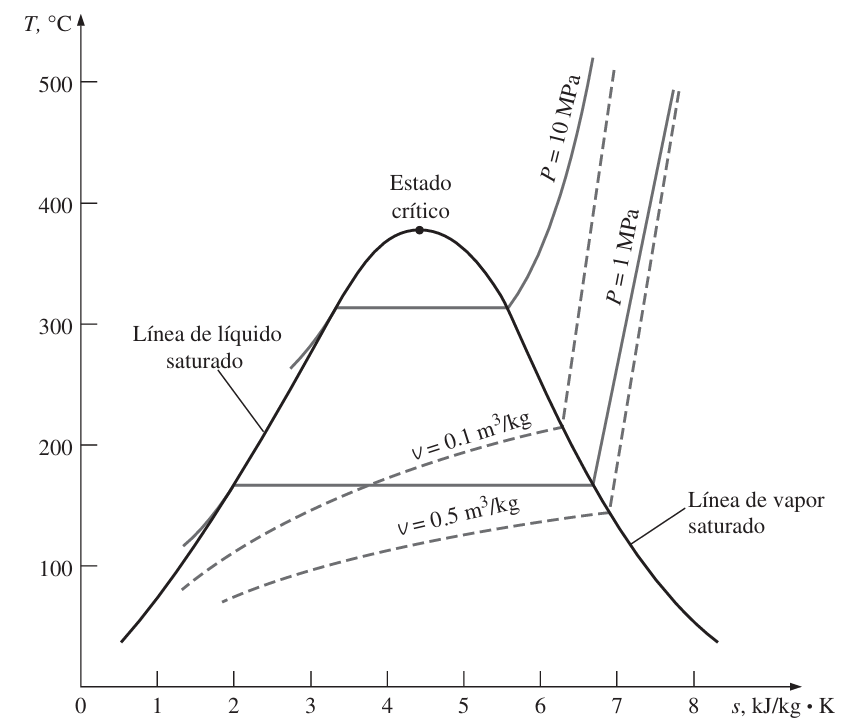
\includegraphics[width = 0.7\linewidth]{Figuras/ANX-01/DiagramaTS.png}
    \caption{Diagrama $T-s$.}\label{FA1-Diagrama T-S.}
\end{figure}

\subsection{Diagrama p-v}

El diagrama $p-v$ se define a partir del volumen específico en las abscisas y la presión específica en las ordenadas. Este diagrama, presente en la figura \ref{FA1-Diagrama p-V.}, permite realizar un análisis simple pero efectivo de la relación entre la presión y el volumen, características fundamentales de un sistema de refrigeración. Además, en dicha gráfica, se visualizan curvas de propiedades constantes.


\begin{figure}[H]
    \centering
    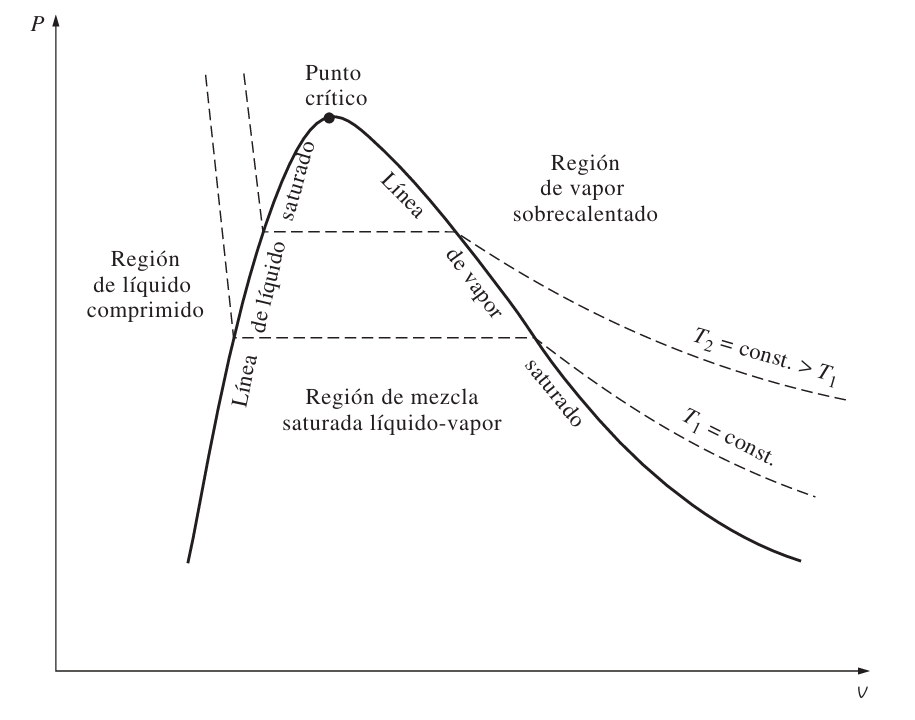
\includegraphics[width = 0.7\linewidth]{Figuras/ANX-01/DiagramaPV.png}
    \caption{Diagrama $p-V$.}\label{FA1-Diagrama p-V.}
\end{figure}

\subsection{Diagrama p-h}

El diagrama $p-h$ consiste en un eje de abscisas que muestra los valores de entalpía, mientras que en sus ordenadas muestra la presión, en la figura \ref{FA1-Diagrama p-h.} se presenta este diagrama. 

Al utilizar el diagrama $p-h$ se presentan dos ventajas interesantes, la primera de ellas es la determinación del aporte o egreso de calor a partir de la diferencia de entalpía, cuando el proceso es isobárico; mientras que la otra ventaja es la fácil determinación de otros parámetros relacionados al sistema a partir de definir el estado como un punto en el diagrama.

\begin{figure}[H]
    \centering
    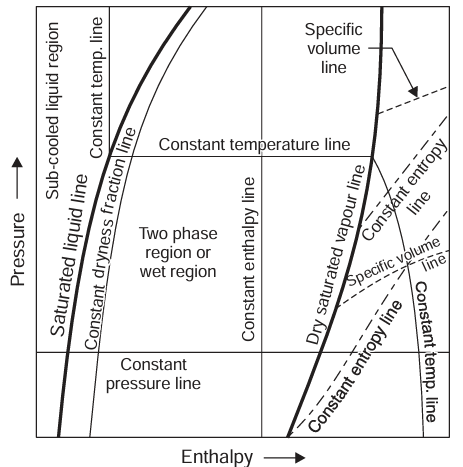
\includegraphics[width = 0.5\linewidth]{Figuras/ANX-01/DiagramaPh.png}
    \caption{Diagrama $p-h$.}\label{FA1-Diagrama p-h.}
\end{figure}



\section{Ciclo Carnot inverso}
\Biblio{\cite[pág. 619 a 620]{Cengel2009termodinamica}}

\begin{defs}
    El \textbf{ciclo Carnot inverso} es un ciclo cuyo fluido de trabajo es vapor de agua y está compuesto por dos isentrópicas y dos isotérmicas. El intercambio de calor se presenta por el cambio de estado del agua.

    El rendimiento, como ciclo de refrigeración, está definido por:

    \begin{equation}\label{EA1-COP ciclo carnot}
        COP_R = \dfrac{1}{\left(T_H/T_L\right)-1}
    \end{equation}

\end{defs}

El ciclo Carnot inverso es un ciclo ideal el cual posee el mayor rendimiento cuando opera entre dos niveles específicos de temperatura. 

Sin embargo, en la práctica el ciclo Carnot no posee un comportamiento ideal en los ciclos de refrigeración. Esto puede explicarse analizando los procesos isotérmicos  y isentrópicos.

\begin{itemize}
    \item El proceso isotérmico es posible no es difícil de lograr, debido a que al mantener una presión y volumen constante, la temperatura se mantiene constante.
    \item El proceso isentrópico no es fácil de lograr en la práctica, ya que la compresión debe realizarse en una mezcla en dos estados (líquido y gaseoso), y la expansión en una turbina que tolere el gran contenido de humedad.
\end{itemize}

\begin{figure}[H]
    \centering
    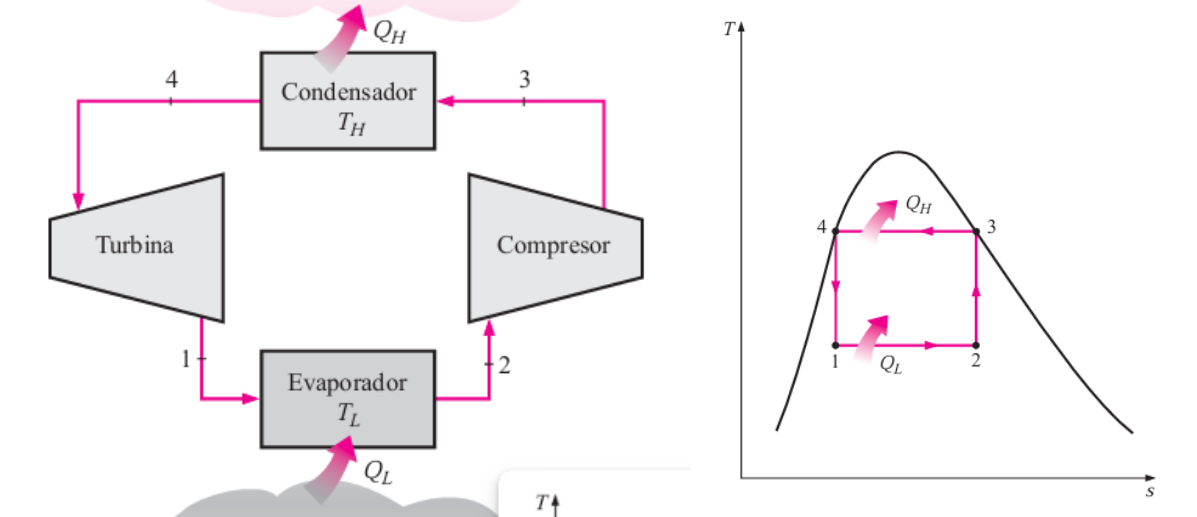
\includegraphics[width = 0.8\linewidth]{Figuras/ANX-01/CICLO_CARNOT.png}
    \caption{Ciclo Carnot inverso.}\label{FA1-Ciclo Carnot inverso}
\end{figure}

\section{Ciclo Rankine inverso}
\Biblio{\cite[pág. 630]{Cengel2009termodinamica} \cite[pág. 738 a 742]{Rajput2011termodinamica}}

\begin{defs}
    El \textbf{ciclo Rankine inverso} es un ciclo cuyo fluido de trabajo es vapor de agua y está compuesto por dos isobaras y una isentrópica y una isoentálpica. El intercambio de calor se presenta por el cambio de estado del agua y la reducción de temperatura del fluido.

    El rendimiento térmico, como ciclo de refrigeración, está definido por:

    \begin{equation}
        COP_R = \dfrac{h_2 - h_1}{h_3 - h_2}
    \end{equation}

\end{defs}

El ciclo Rankine inverso es un ciclo que posee un rendimiento próximo al de Carnot inverso debido a ser un derivado de él.

Este ciclo tiene como objetivo solucionar los inconvenientes en el ciclo de Carnot inverso que se presentaban principalmente en los procesos isentrópicos. El ciclo Rankine inverso propone como solución la compresión del fluido en forma de vapor completamente, lo que evita el uso de equipos complejos que toleren mezclas sólidas y líquidas. 

\begin{figure}[H]
    \centering
    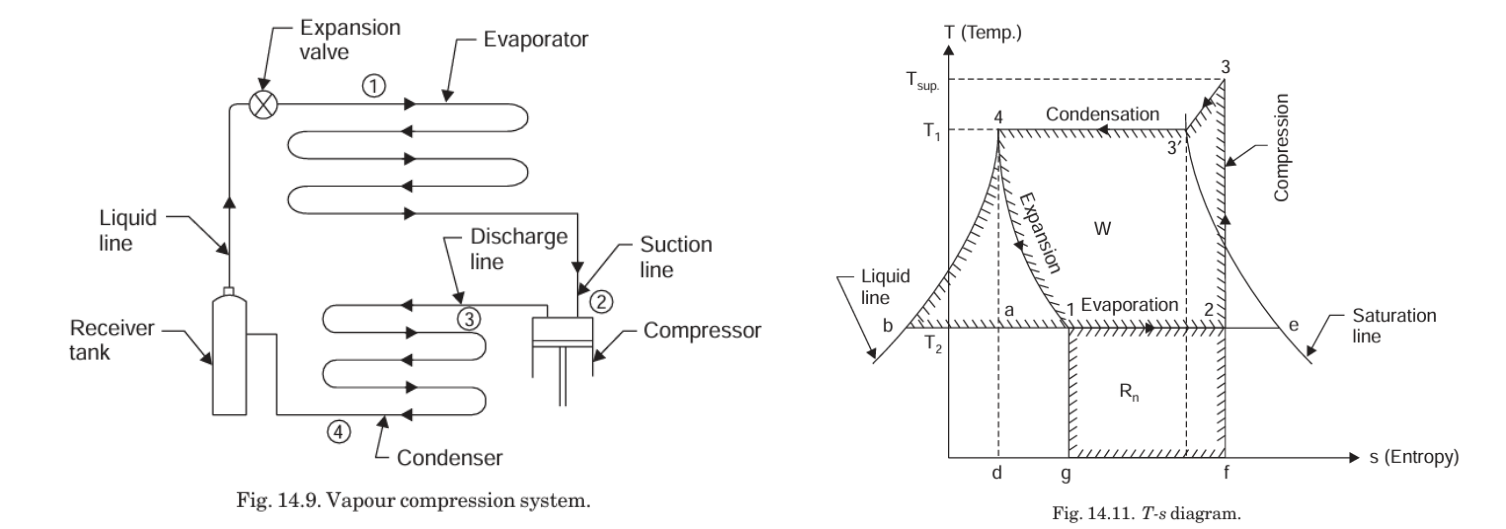
\includegraphics[width = \linewidth]{Figuras/ANX-01/CICLO_RANKINE.png}
    \caption{Ciclo Rankine inverso.}\label{FA1-Ciclo Rankine inverso}
\end{figure}

Este sistema, de forma simple, se compone de los siguientes procesos y elementos que los realizan:

\begin{enumerate}
    \item Compresión por compresor: el compresor cumple la función de remover el vapor del evaporador y aumentar la temperatura y la presión hasta un punto tal que el vapor se pueda condensar con el medio de condensación disponible. Esta compresión es idealmente isentrópica.
    \item Condensación por condensador: el condensador tiene como función proporcionar una superficie de transferencia de calor a través de la que el calor pasa del vapor refrigerante caliente al medio de condensación. Este proceso se supone a presión constante.
    \item Expansión con válvula de expansión: la válvula dosifica la cantidad apropiada de refrigerante hacia el evaporador con el fin de reducir la presión del líquido entrante al evaporador de manera uqe el líquido que se vaporizará en el evaporadora ala temperatura baja deseada tomará una suficiente cantidad de calor. Este procedimiento es isentálpico.
    \item Vaporización en evaporador: el evaporador, así como el condensador, proporciona una superficie de transferencia de calor a través de la cual el calor puede pasar del espacio refrigerado hacia el refrigerante vaporizado.
\end{enumerate}

Tomando el diagrama del ciclo Rankine inverso de la figura \ref{FA1-Ciclo Rankine inverso}, donde la compresión del vapor se continúa después de que se ha secado, el vapor estará sobrecalentado. EL vapor entra al compresor en la condición 2 y se comprime hasta 3 donde se sobrecalienta hasta la temperatura $T_3$. Luego entra al condensador. Aquí, el vapor sobrecalentado se enfría hasta la temperatura $T_1$ y luego se condensa a tempeartura constante a lo largo de la línea $3´-4$. 

\section{Ciclo Brayton inverso}
\Biblio{\cite[pág. 641]{Cengel2012termodinamica}}

\begin{defs}
    El \textbf{ciclo Brayton inverso} es un ciclo cuyo fluido de trabajo es comúnmente un gas y está compuesto por dos isentrópicas y dos isobaras.

    El rendimiento térmico, como ciclo de refrigeración, está definido por:

    \begin{equation}\label{EA1-Rendimiento de ciclo Brayton inverso}
        COP_R = \dfrac{h_4 - h_1}{h_1+ h_3 - (h_4 + h_1)}
    \end{equation}
\end{defs}

En detalle se considera el ciclo de refrigeración de gas que se muestra en la figura \ref{FA1-Ciclo Brayton Inverso}. Los alrededores están a una temperatura $T_3$ y el espacio refrigerado se va mantener a una temperatura $T_1$. El gas se comprime durante el proceso $1-2$. El gas a presión y temperatura altas en estado 2 se enfría después a presión constante hasta $T_3$ al rechazar calor hacia los alrededores. Esto es seguido por un proceso de expansión en una turbina, durante el cual la temperatura del gas disminuye hasta $T_4$. Por último, el gas frío absorbe el valor del espacio refrigerado hasta que su temperatura se eleva hasta $T_1$.

\begin{figure}[H]
    \centering
    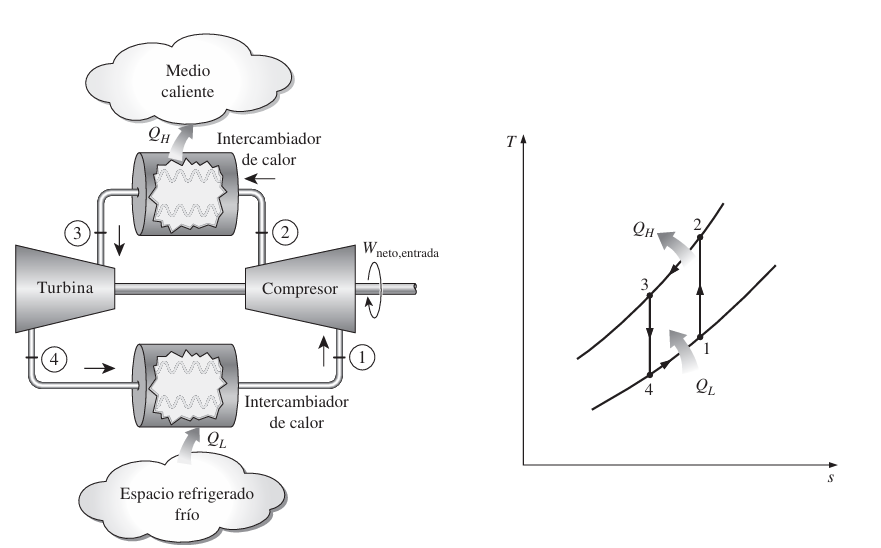
\includegraphics[width = 0.9\linewidth]{Figuras/ANX-01/CICLO_BRAYTON.png}
    \caption{Ciclo Brayton inverso.}\label{FA1-Ciclo Brayton Inverso}
\end{figure}

Todos los procesos recién descritos son internamente reversibles y el ciclo ejecutado es el ciclo ideal de refrigeración de gas. En los ciclos reales de refrigeración de gas, los procesos de compresión y expansión se desviarán de los isentrópicos, y $T_3$ será más alta que la temperatura ambiente, al menos que el intercambiador de calor sea infinitamente largo.
